\section{PCBs Made With LibrePCB}

\begin{frame}{\secname}

  Some PCBs made by the LibrePCB community \faChild\faChild\faChild

  \begin{center}
    \begin{tikzpicture}
        \node (img1)
        {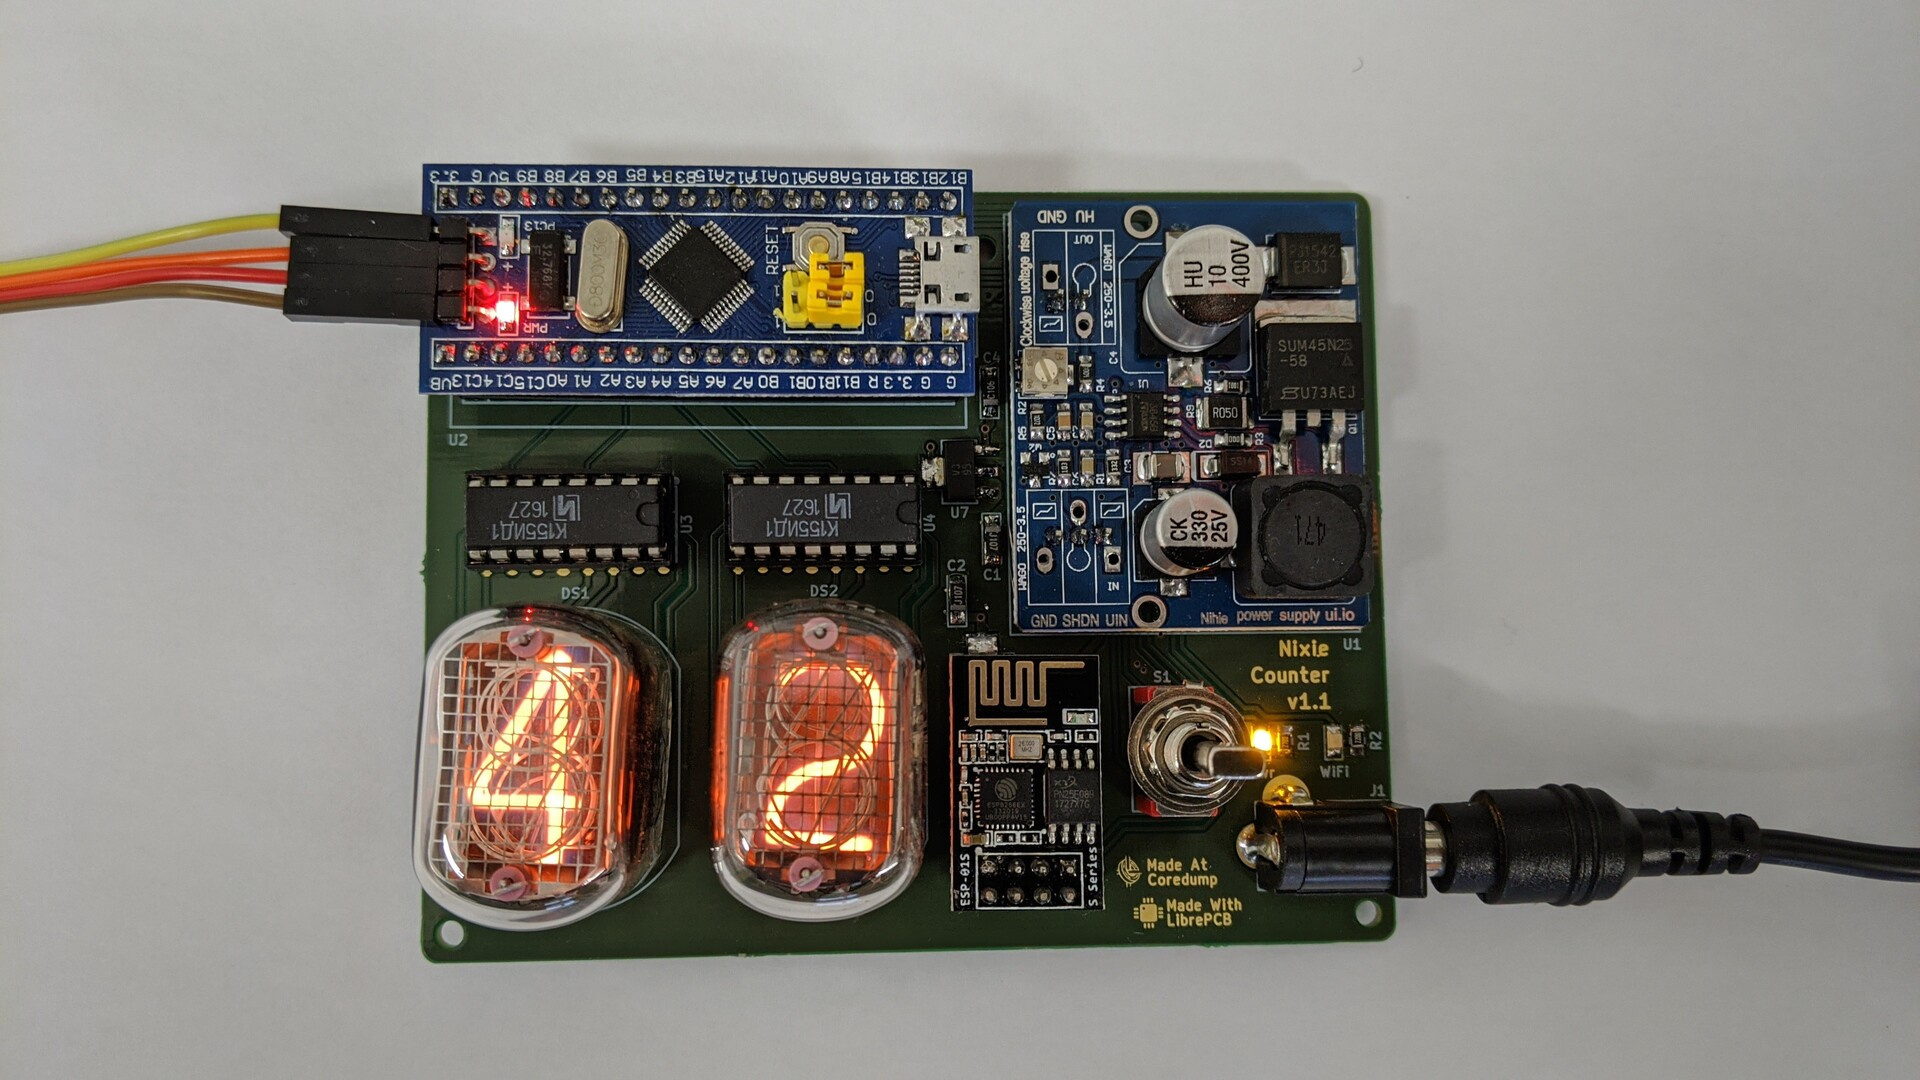
\includegraphics[height=5.5cm]{images/madewithlibrepcb_1.jpeg}};
    \end{tikzpicture}

    \tiny Source:
    \url{https://librepcb.discourse.group/t/projects-madewithlibrepcb/99}
  \end{center}

\end{frame}

\note{
  Here are some of the PCBs created by the community, this might help to
  see what LibrePCB is able to do.\\

  This is a counter with nixie tubes
}

\begin{frame}[noframenumbering]{\secname}

  Some PCBs made by the LibrePCB community \faChild\faChild\faChild

  \begin{center}
    \begin{tikzpicture}
        \node (img2)
        {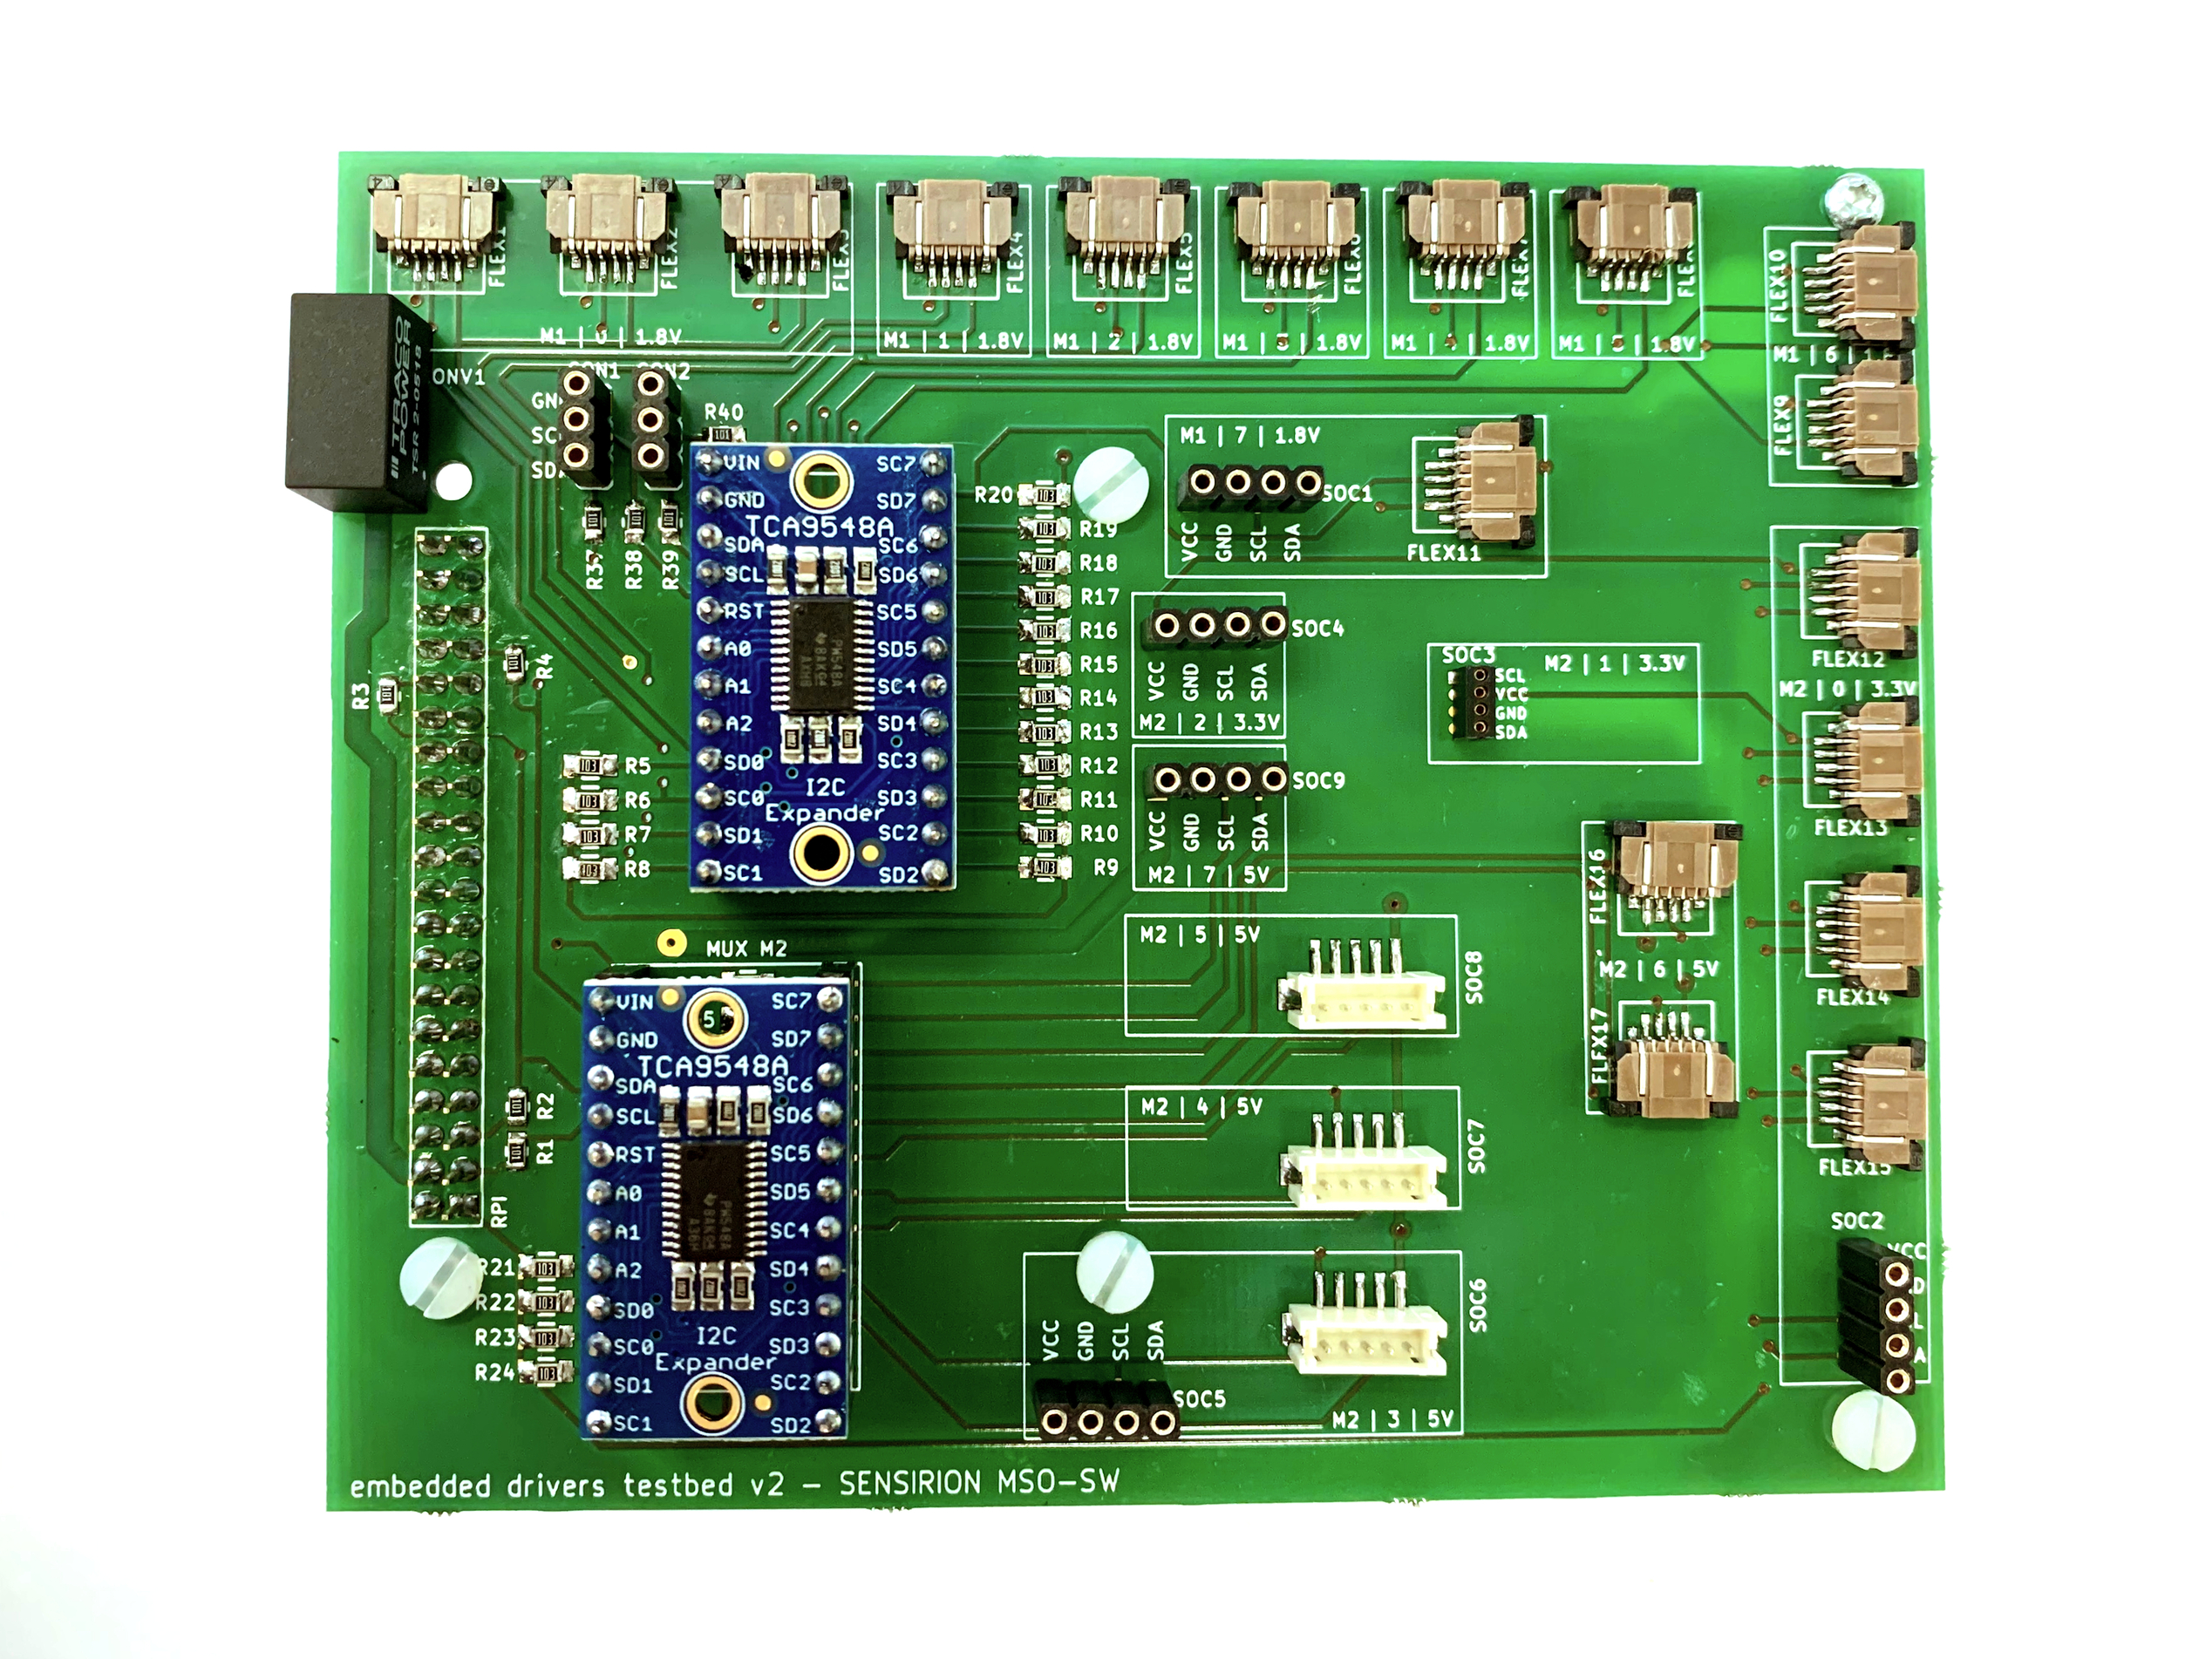
\includegraphics[height=5.5cm]{images/madewithlibrepcb_5.jpeg}};
    \end{tikzpicture}

    \tiny Source:
    \url{https://librepcb.discourse.group/t/projects-madewithlibrepcb/99}
  \end{center}

\end{frame}

\note{
  A raspberry pi shield to connect sensors
}

\begin{frame}[noframenumbering]{\secname}

  Some PCBs made by the LibrePCB community \faChild\faChild\faChild

  \begin{center}
    \begin{tikzpicture}
        \node (img3)
        {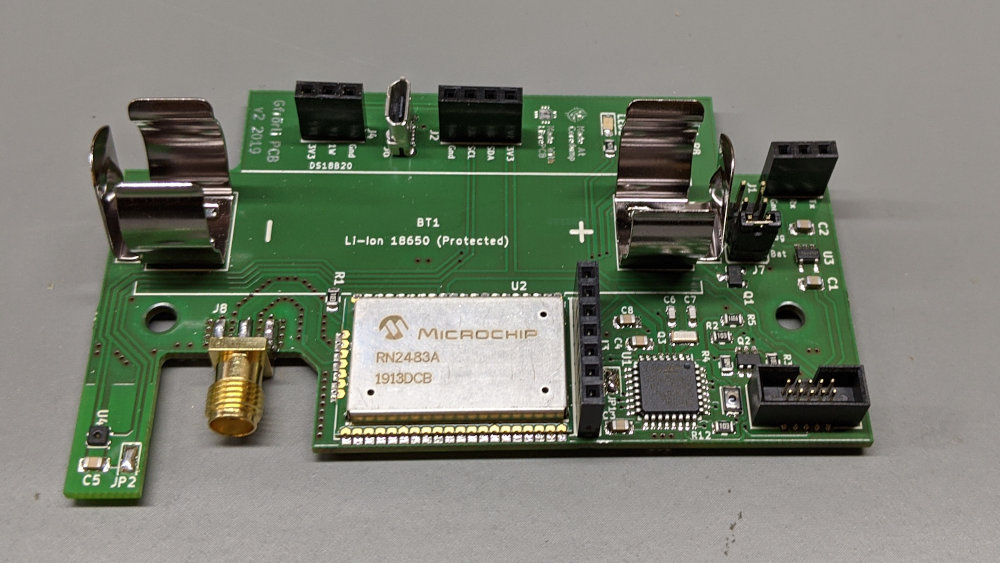
\includegraphics[height=5.5cm]{images/madewithlibrepcb_2.jpeg}};
    \end{tikzpicture}

    \tiny Source:
    \url{https://librepcb.discourse.group/t/projects-madewithlibrepcb/99}
  \end{center}

\end{frame}

\note{
  A water temperature sensor with LoraWAN
}

\begin{frame}[noframenumbering]{\secname}

  Some PCBs made by the LibrePCB community \faChild\faChild\faChild

  \begin{center}
    \begin{tikzpicture}
        \node (img4)
        {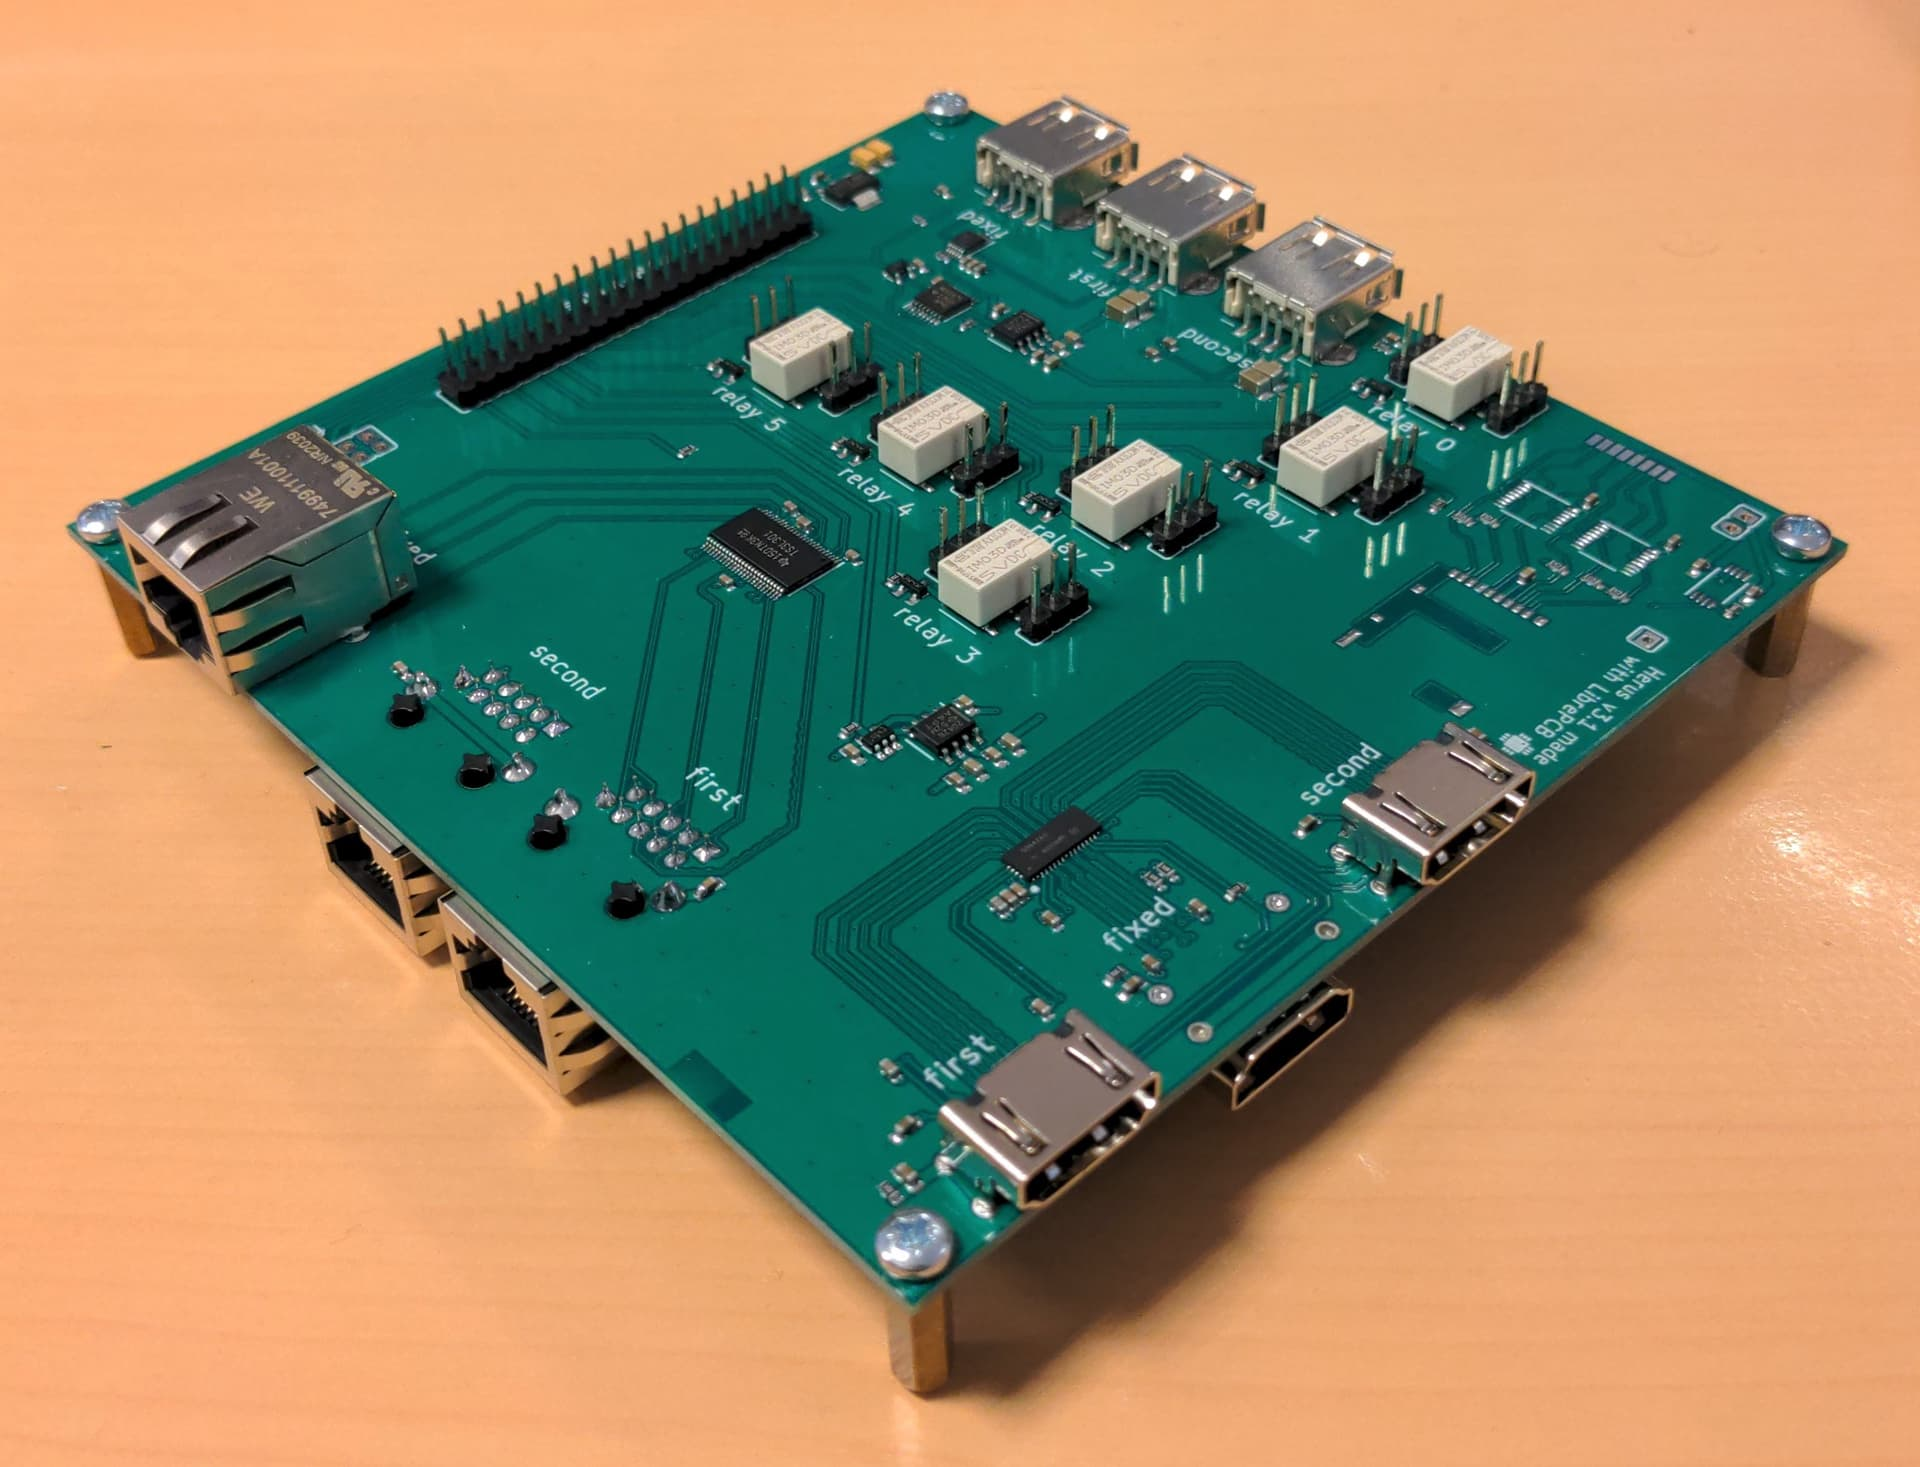
\includegraphics[height=5.5cm]{images/madewithlibrepcb_4.jpeg}};
    \end{tikzpicture}

    \tiny Source:
    \url{https://librepcb.discourse.group/t/projects-madewithlibrepcb/99}
  \end{center}

\end{frame}

\note{
  An expansion board for single board computers
}

\begin{frame}[noframenumbering]{\secname}

  Some PCBs made by the LibrePCB community \faChild\faChild\faChild

  \begin{center}
    \begin{tikzpicture}
        \node (img5)
        {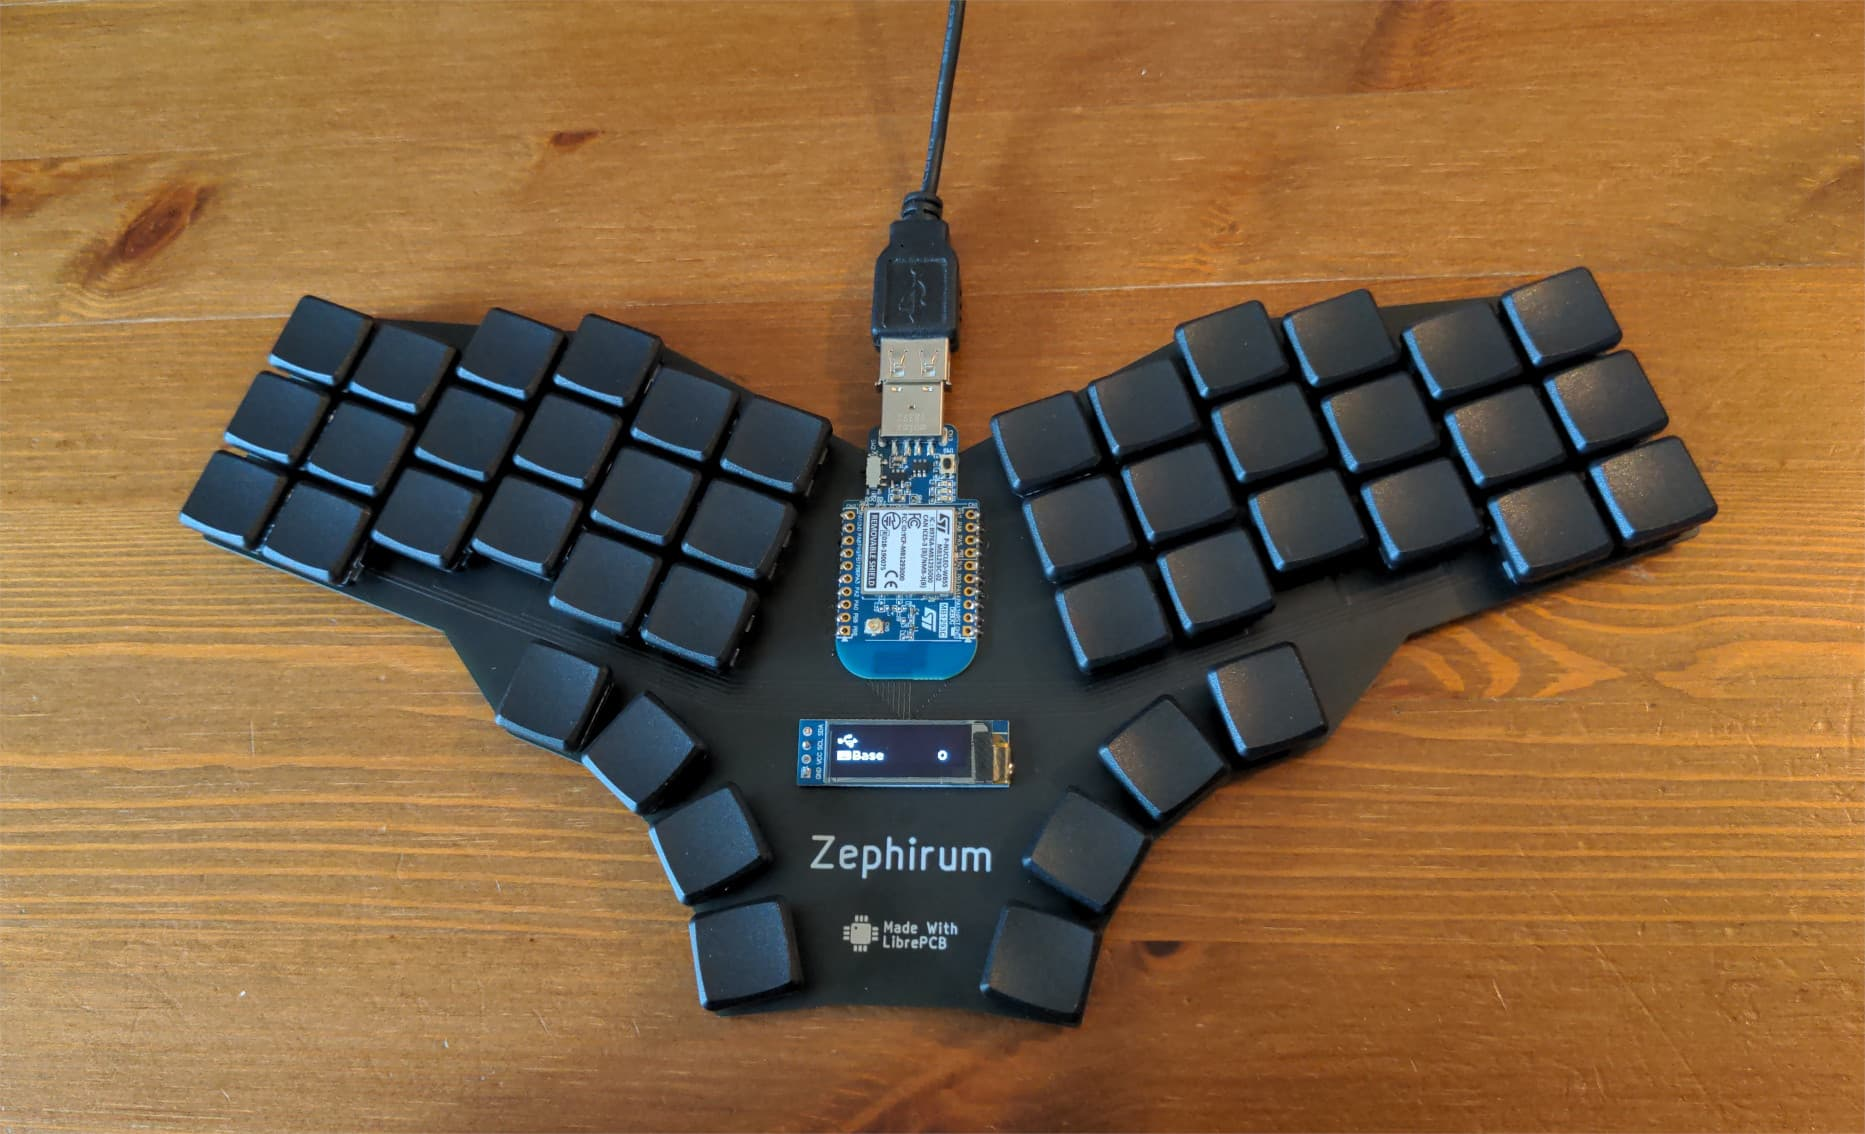
\includegraphics[height=5.5cm]{images/madewithlibrepcb_3.jpeg}};
    \end{tikzpicture}

    \tiny Source:
    \url{https://librepcb.discourse.group/t/projects-madewithlibrepcb/99}
  \end{center}

\end{frame}

\note{
  Or a keyboard.\\

  These projects were posted by LibrePCB users in our forum.
  It's always cool to see what LibrePCB is used for, so if you created a
  PCB with it, it would be great to share it in our forum as well.
}
